\documentclass[a4paper,10pt]{article}
\usepackage[utf8]{inputenc}
\usepackage{amsmath}
\usepackage{xfrac}
%\usepackage[demo]{graphicx}
\usepackage[caption = false]{subfig}
\usepackage{float}
\usepackage[a4paper, total={7.5in, 10in}]{geometry}
\usepackage{longtable}
\usepackage{dcolumn,booktabs}
\usepackage[table]{xcolor}
\usepackage{listings}
\lstset{
breaklines=true
}
%http://tex.stackexchange.com/questions/116534/lstlisting-line-wrapping
\usepackage{hyperref}
\hypersetup{
    colorlinks=true,
    linkcolor=blue,
    citecolor=blue
}

\lstset{language=[77]Fortran,
  basicstyle=\ttfamily,
  keywordstyle=\color{red},
  commentstyle=\color{green},
  morecomment=[l]{!\ }% Comment only with space after !
}

\usepackage{color}
 
\definecolor{codegreen}{rgb}{0,0.6,0}
\definecolor{codegray}{rgb}{0.5,0.5,0.5}
\definecolor{codepurple}{rgb}{0.58,0,0.82}
\definecolor{backcolour}{rgb}{0.95,0.95,0.92}
 
\lstdefinestyle{mystyle}{
    backgroundcolor=\color{backcolour},   
    commentstyle=\color{codegreen},
    keywordstyle=\color{magenta},
    numberstyle=\tiny\color{codegray},
    stringstyle=\color{codepurple},
    basicstyle=\footnotesize,
    breakatwhitespace=false,         
    breaklines=true,                 
    captionpos=b,                    
    keepspaces=true,                 
    numbers=left,                    
    numbersep=5pt,                  
    showspaces=false,                
    showstringspaces=false,
    showtabs=false,                  
    tabsize=2
}
 
\lstset{style=mystyle}

%opening

\title{Homework 5 \\
\textbf{Simultaneous system of two equations}}
\author{Arvind Balasubramanian}
\date{}

\begin{document}
\maketitle
\section*{Python code and analysis}
\begin{lstlisting}[language=python]
import numpy as np

def F(x,y):
    return 2*(x**3.0) - (y**2.0) - 1

def G(x,y):
    return x*(y**3.0) - y - 4

def partialx(function,x0,y0,stepsize):
    """
    Returns partial first derivative of the function "function" at the point x0,y0 with respect to x by considering points, one and two steps on either side of x0.
    The Accuracy is of order (stepsize)^4.
    """
    return (function(x0 - 2*stepsize, y0) - 8*function(x0 - stepsize, y0) + 8*function(x0 + stepsize, y0) - function(x0 + 2*stepsize, y0))/(12*stepsize)

def partialy(function,x0,y0,stepsize):
    """
    Returns partial first derivative of the function "function" at the point x0,y0 with respect to y by considering points, one and two steps on either side of y0.
    The Accuracy is of order (stepsize)^4.
    """
    return (function(x0, y0 - 2*stepsize) - 8*function(x0, y0 - stepsize) + 8*function(x0, y0 + stepsize) - function(x0, y0 + 2*stepsize))/(12*stepsize)

def det(a,b,c,d):
    return a*d - b*c

def Jacobian(F,G,x,y,stepsize):
    """
    Returns the jacobian of F and G at the point x and y
    """

    a = partialx(F,x,y,stepsize)
    b = partialy(F,x,y,stepsize)
    c = partialx(G,x,y,stepsize)
    d = partialy(G,x,y,stepsize)

    return det(a,b,c,d)


def NewtonSolver(F,G,x0,y0,stepsize):
    """
    Solves the system of equations F(x,y) = 0 and G(x,y) = 0 using the Newton Raphson method
    """
     J = Jacobian(F,G,x0,y0,stepsize)
     s = 0
     if (J == 0):
         return "Warning! : Jacobian is zero! Please enter a better guess!"
     else:
         s += 1
         h = (-1.0/J)*det(F(x0,y0),partialy(F,x0,y0,stepsize),G(x0,y0),partialy(G,x0,y0,stepsize))
         k = (-1.0/J)*det(partialx(F,x0,y0,stepsize),F(x0,y0),partialx(G,x0,y0,stepsize),G(x0,y0))
         x1 = x0 + h
         y1 = y0 + k
         while((abs(x1-x0) > 10**(-8)) and (abs(y1-y0) > 10**(-8))):
             x0 = x1
             y0 = y1
             J = Jacobian(F,G,x0,y0,stepsize)
             if (J == 0):
                 return "Warning! : Jacobian is zero! Please enter a better guess!"
             else:
                 h = (-1.0/J)*det(F(x0,y0),partialy(F,x0,y0,stepsize),G(x0,y0),partialy(G,x0,y0,stepsize))
                 k = (-1.0/J)*det(partialx(F,x0,y0,stepsize),F(x0,y0),partialx(G,x0,y0,stepsize),G(x0,y0))
                 x1 = x0 + h
                 y1 = y0 + k
                 s += 1
                 print(h,k)
                 print("step : ",s)
     return x1, y1, s

x_guess = 0
y_guess = 1.0

x1, y1, s = NewtonSolver(F,G,x_guess,y_guess,10**(-8))
\end{lstlisting}

\pdfsuppresswarningpagegroup=1

\vspace{80pt}
\newpage
\section*{Plots}
The title of the plots signifies how many iterations it took to converge to the solution. The chosen initial conditions are tabulated in the legend.

\begin{figure}[H]
\centering
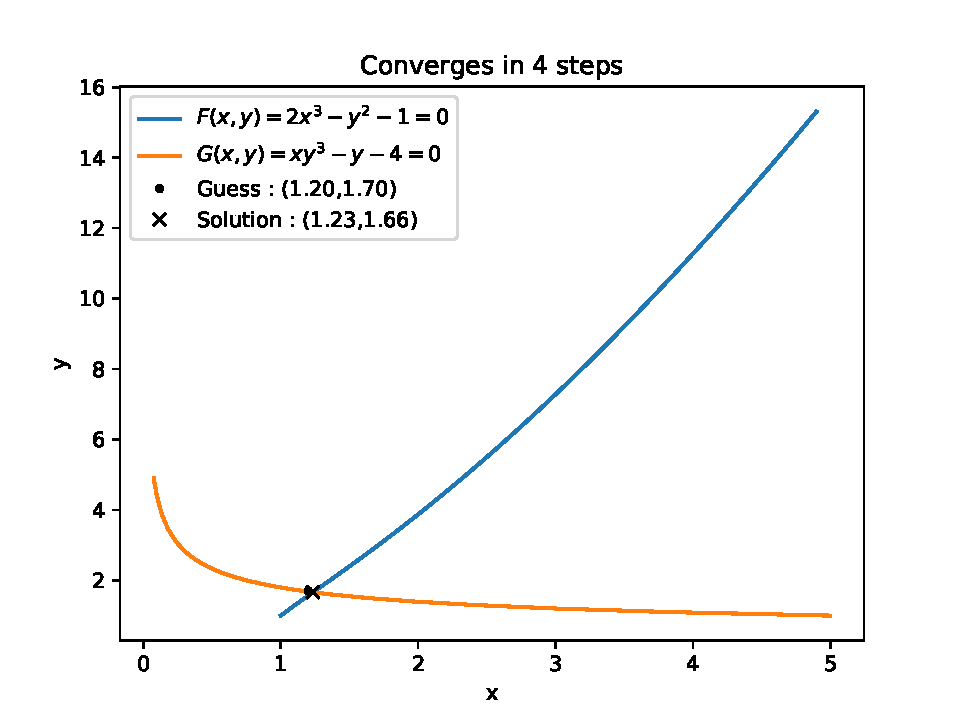
\includegraphics[width=0.9\textwidth]{Figure_1} 
\end{figure}

\begin{figure}[H]
\subfloat[]{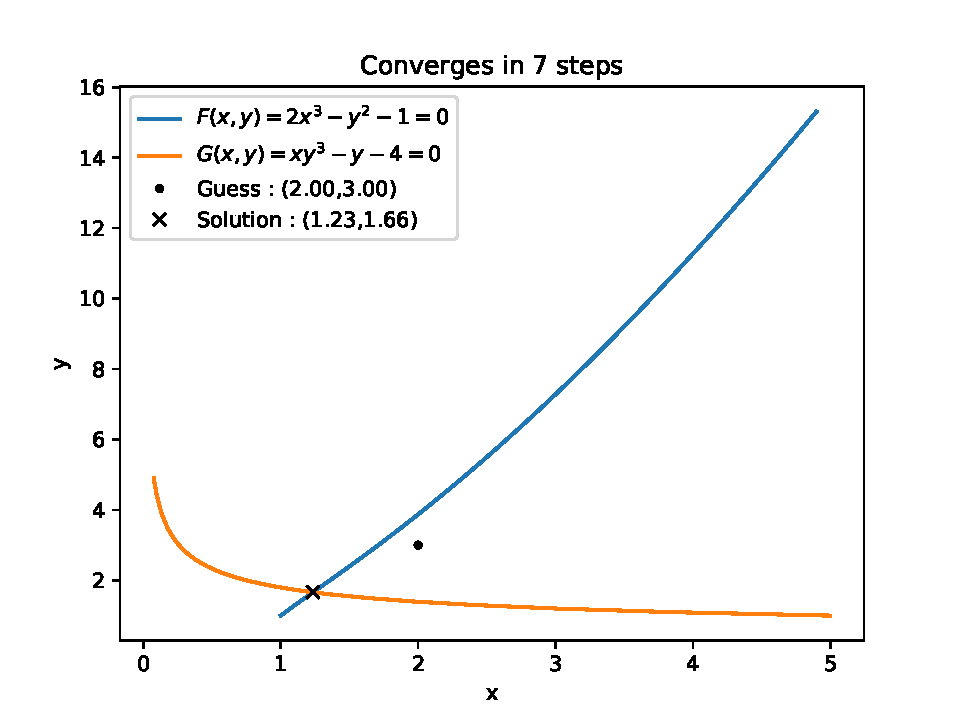
\includegraphics[width = 0.5\textwidth]{Figure_2}} 
\subfloat[]{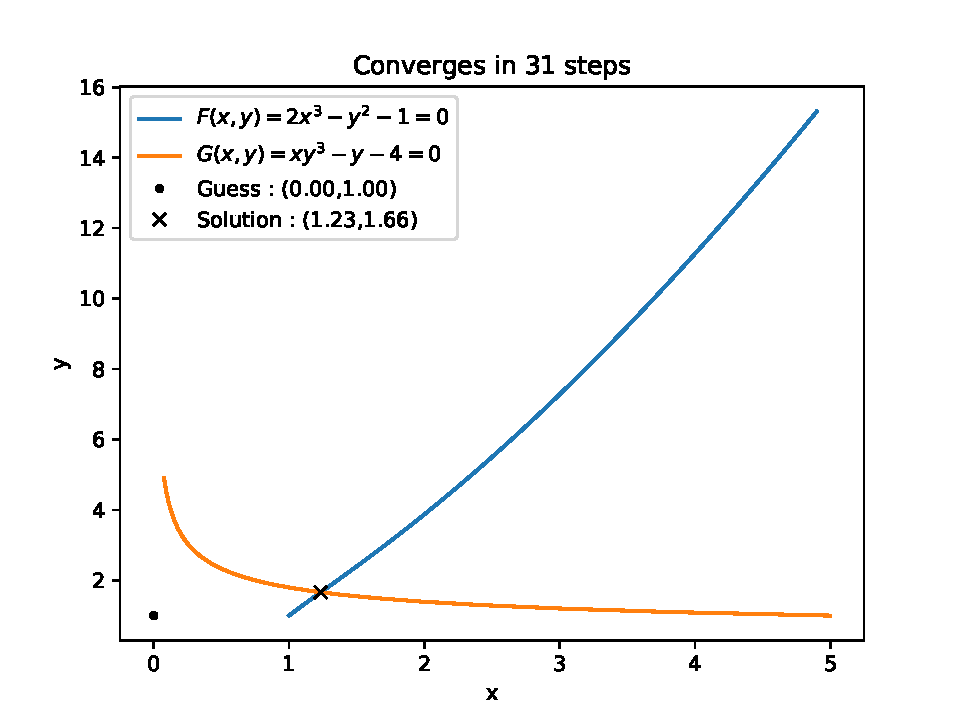
\includegraphics[width = 0.5\textwidth]{Figure_3}}
\end{figure}


\end{document}
